%%%%%%%%%%%%%%%%%%%%%%%%%%%%%%%%%%%%%%%%%%%%%%%%%%%%%%%%%%%%%%%%%%%%%%%%
\chapter{Representation Learning for Natural Language}
\label{sec:rw_repl_nl}
%%%%%%%%%%%%%%%%%%%%%%%%%%%%%%%%%%%%%%%%%%%%%%%%%%%%%%%%%%%%%%%%%%%%%%%%

\begin{center}
  \begin{minipage}{0.7\textwidth}
    \textit{The performance of machine learning methods is heavily
dependent on the choice of data representation (or
features) on which they are applied.} 
\begin{flushright}- \citet{bengio_repr} \end{flushright}
  \end{minipage}
\end{center}

It is often stated informally that 
$$
\text{Machine Learning} = \text{Representation} + \text{Objective} + \text{Optimization}
$$
The \textit{representation} part of machine learning consists in building numerical features from the data that will easily allow a prediction to be made by a parameterized model. The conformity of this prediction to the expected result can then be evaluated by an \textit{objective} function. Finally, an \textit{optimization} algorithm is used to modify the parameterized model (and possibly the representations themselves) in order to maximize (or minimize) the objective function on the provided data points. As most parameterized models rely on numerical operations, which are often algebraic transformations, real-valued vectors (sometimes viewed as matrices or tensors) are a particularly well-suited choice for representations, although some methods yield integer-based representations \citep{10.5555/3295222.3295378}.

For tabular data, choosing representations to feed a statistical or neural model is straightforward, as they are readily available in a numerical format and can be vectorized directly. However, for modalities such as natural language, the representation step is crucial and raises various questions. Text can be seen as a sequence of symbols that follow some hierarchical patterns \citep{longacre}, which makes harder to translate to vector representations, especially as these underlying patterns are complex and brittle to subtle changes. Even when the notion of atomic units is defined (see \Cref{subsec:rw_lm_tokenization}), some properties of language demand peculiar attention before tensor representations can be extracted and used in machine learning pipelines.

Firstly, written natural language is discrete. Each atomic unit is a discrete symbol that cannot trivially be converted to a real-valued representation in a metric space that is meaningful with respect to the objectives of the models. As a consequence, the only notion of distance that can be immediately derived from raw text is purely lexical, with notable examples being Levenshtein distance \citep{levenshtein1966binary} and alternatives \citep{hamming, jaro}.

Secondly, textual data is sequential, which complexifies the possible nature of tasks and the granularity of the represented objects compared to pure tabular data. For instance, some models may be designed to classify words, and others to cope with document-level tasks. This implies that textual information of different nature and/or shape (e.g. two documents with different lengths or languages) may need to be represented in similar vector spaces so that a machine learning model can perform predictions about these different pieces of information.


In this section, we present works that address the question learning representations from textual data of different nature, from word-level to document-level, and we compare the objectives and conclusions drawn from these different lines of work.




%%%%%%%%%%%%%%%%%%%%%%%%%%%%%%%%%%%%%%%%%%%%%%%%%%%%%%%%%%%%%%%%%%%%%%%%
\section{Statistical Methods}

Chronologically, the first NLP tasks that benefitted from learning  strong representations were sentence-level and document-level classification tasks \citep{baharudin2010review}, particularly in the field of Information Retrieval \citep{chowdhury2010introduction}. 

\subsection{Counting Methods}

A naive approach to document representation, called \textit{bag-of-words} (BoW), consists in counting the words and using a histogram as a vector representation. Based on the token sequence framework introduced in \Cref{sec:rw_lm}, we consider a document $D$ as a sequence of tokens $(w_t)_{t \in {L_D}}$, and we define its bag-of-word representation $x \in \mathbb{N}^V$:
$$
x_w = \sum_{i=1}^{L_D} \mathbf{1}_{w_i = w}
$$

This representation can be normalized for more consistency across documents. A known limitation of the BoW approach is its failure to properly cope with the extremely unbalanced distribution of words in natural language. \citet{zipf_psycho-biology_1935} shows that the unigram frequency of words in the English language tend to follow a power law of mass function:
$$
f_s(w_i) = \frac{1}{H_{s, V}} \frac{1}{i^s}
$$
where words $(w_i)$ are sorted by frequency, and $H_{s, V}$ is a normalization term. As a result, BoW representations are not easily distinguishable as they tend to provide higher values to words that are generally frequent (e.g. stop words) and do not shed light on the specificity of the document they belong to.

To alleviate this issue, \citet{tf_idf} correct the word count by using a term that takes a global rate of occurence of the word into account. Their method, called \textit{Text Frequency - Inverse Document Frequency} (TF-IDF), computes a document representation $x^i \in \mathbb{R}^V$ in a document corpus $(D_i)_{i \in [1, \mathcal{D}]}$:
$$
x^i_w = \frac{\sum_{i=1}^{L_{D_i}} \mathbf{1}_{w_i = w}}{|D_i|} \cdot \frac{\mathcal{D}}{\sum_{j=1}^{\mathcal{D}} \mathbf{1}_{w \in D_j}}
$$

The first term corresponds to Text-Frequency, and can take other forms (e.g. log-regularization). The second term is Inverse-Document-Frequency and computes the rate of documents that contain the word $w$. This technique yields more \textit{expressive} representations as resulting vectors better capture the specificity of different documents \citep{ramos2003using}.

\subsection{Topic Modeling}

The representations obtained with aforementioned methods rely on token counting, and usually are high-dimensional sparse vectors. This incentivizes the exploration of compression techniques, that would yield denser vectors in lower-dimensional spaces, which should improve the efficiency and memory requirements of the models based on these representations.

Both with BoW and TF-IDF, the resulting representations can indeed be automatically compressed to lower-dimensional vectors at corpora level using \textit{Latent Semantic Analysis} (LSA) \citep{deerwester1990indexing}. To do so, LSA relies on the Singular Value Decomposition (or SVD) of the matrix of document representations\footnote{In the case of BoW, this matrix is also called the \textit{Term-Document} matrix.} $X \in \mathbb{R}^{\mathcal{D} \times V}$ to identify components that are shared across documents.

SVD is a matrix factorization technique that can be applied to real matrices $M$ of any shape $m \times n$ and leads to the following decomposition:
$$
M = U \Sigma V^T
$$
where $U$ and $V$ are square matrices of shapes $m \times m$ and $n \times n$ respectively, and $\Sigma$ is an $m \times n$ diagonal matrix of coefficients:
\begin{equation*}
  \Sigma_{ij} = \begin{cases}
    \sigma_i \text{ if } i=j \\
    0 \text{ else.}
  \end{cases}
\end{equation*}
The coefficients $\sigma_i$ are the singular values of $M$, ie. they are the non-negative square roots of the eigenvalues of $M^TM$.

LSA performs a form of Principal Component Analysis on $X$ by organizing the dimensions of the SVD to ensure that $\sigma_i$ are sorted in decreasing order, and by truncating the shapes of $U$, $\Sigma$ and $V$ to match a target dimension $d$. This truncation creates compact representations of the documents as the columns of the truncated $V_{:d}$. The principal components $U_{:d}$ can also be seen as \textit{topics}, as they contain the underlying direction of the representations that better capture the information in the documents. For instance, in the case of BoW, these vectors can be expected to separate word distributions that are characteristic of certain thematics of the documents in the corpus.

The idea of extracting topics from document corpora has been thoroughly explored in the field of \textit{topic modeling} \citep{churchill2022evolution}, especially via the widely used technique called \textit{Latent Dirichlet Allocation} \citep{lda}. This technique builds a statistical model using explicit topics as token distributions and distributions over these topics to model documents.



\subsection{Co-occurence Matrices}

The key concept for most statistical methods used to obtain word-level representations is the distributional hypothesis \citep{harris1954distributional} that states that words are characterized by the words that appear in their context. \citep{weaver-1952-translation} introduces \textit{statistical semantics}, a field that employs statistical methods to analyze word meanings in natural languages. A straightforward application of these theories to the document representation framework consists in considering the columns of $X$ as useful token-level representations, as tokens that appear in the same documents should convey similar meanings.

The notion of context can be extended to broader definitions to build a term-term matrix which for instance counts occurrences of token $w_i$ in a $k$-token window surrounding all occurrences of $w_j$ in a text corpus. 

Nevertheless, similarly to BoW, these purely counting-based representations are distorted by the peculiar nature of the Zipfian distribution of tokens in natural language. This incentivizes the use of pointwise mutual information \citep{shannon_mi} as a measure of the level of dependency between two tokens. For a context defined by $\mathcal{C}$, the pointwise mutual information (PMI) between two tokens co-occurring $w_i$ and $w_j$ is:
$$
\text{PMI}(w_i, w_j) = \log_2 \frac{P(w_i \in \mathcal{C}(w_j))}{P(w_i) \cdot P(w_j)}
$$
The PMI captures the rate of co-occurrence of tokens $w_i$ and $w_j$ over their rate of appearance, which regularizes the dependency score for high-frequency tokens, and make semantically meaningful interactions stand out.

A commonly used alternative is Positive PMI (or PPMI):
$$
\text{PPMI}(w_i, w_j) = \max (0, \log_2 \frac{P(w_i \in \mathcal{C}(w_j))}{P(w_i) \cdot P(w_j)})
$$
PPMI avoids considering the PMI where it is negative, that is where tokens tend to particularly \textit{not} co-occur, which is difficult to estimate safely from a statistical perspective, especially for rare tokens.

LSA can also be used to obtain token-level embeddings, by computing the SVD on $X^T$ and using $U \in \mathbb{R}^{V \times d}$ as a look-up table for token representations.


%%%%%%%%%%%%%%%%%%%%%%%%%%%%%%%%%%%%%%%%%%%%%%%%%%%%%%%%%%%%%%%%%%%%%%%%
\section{Machine Learning Methods}

As computational capabilities improved over the years, machine learning approaches were increasingly studied in Natural Language Processing \citep{billingsley-curran-2012-improvements,cho-etal-2014-learning}.

\subsection{Word2Vec} In the domain of word-level representation, a pioneering work is Word2Vec \citep{word2vec}. Building upon Neural Network Language Models \citep{bengio2000neural}, the authors build neural networks without intermediate layers and train them on one of two tasks that are closely related with language modeling. The first task, \textit{continuous bag-of-word} or CBOW, consists in predicting a token based on a bidirectional short context window, using the classical language modeling framework and a more efficient hierarchical softmax \citep{pmlr-vR5-morin05a}. The second task, called \textit{Skip-gram}, mirrors the first one by using the central token to predict the tokens from the short context window, and apply a language modeling objective at each of the predicted positions. In both cases, the input embeddings of the models are used as the token representations. The authors conduct experiments with these representations and conclude that they convey higher semantic and syntactic information compared with using the intermediate representations of NNLMs.
\begin{figure}[ht]
  \centering
  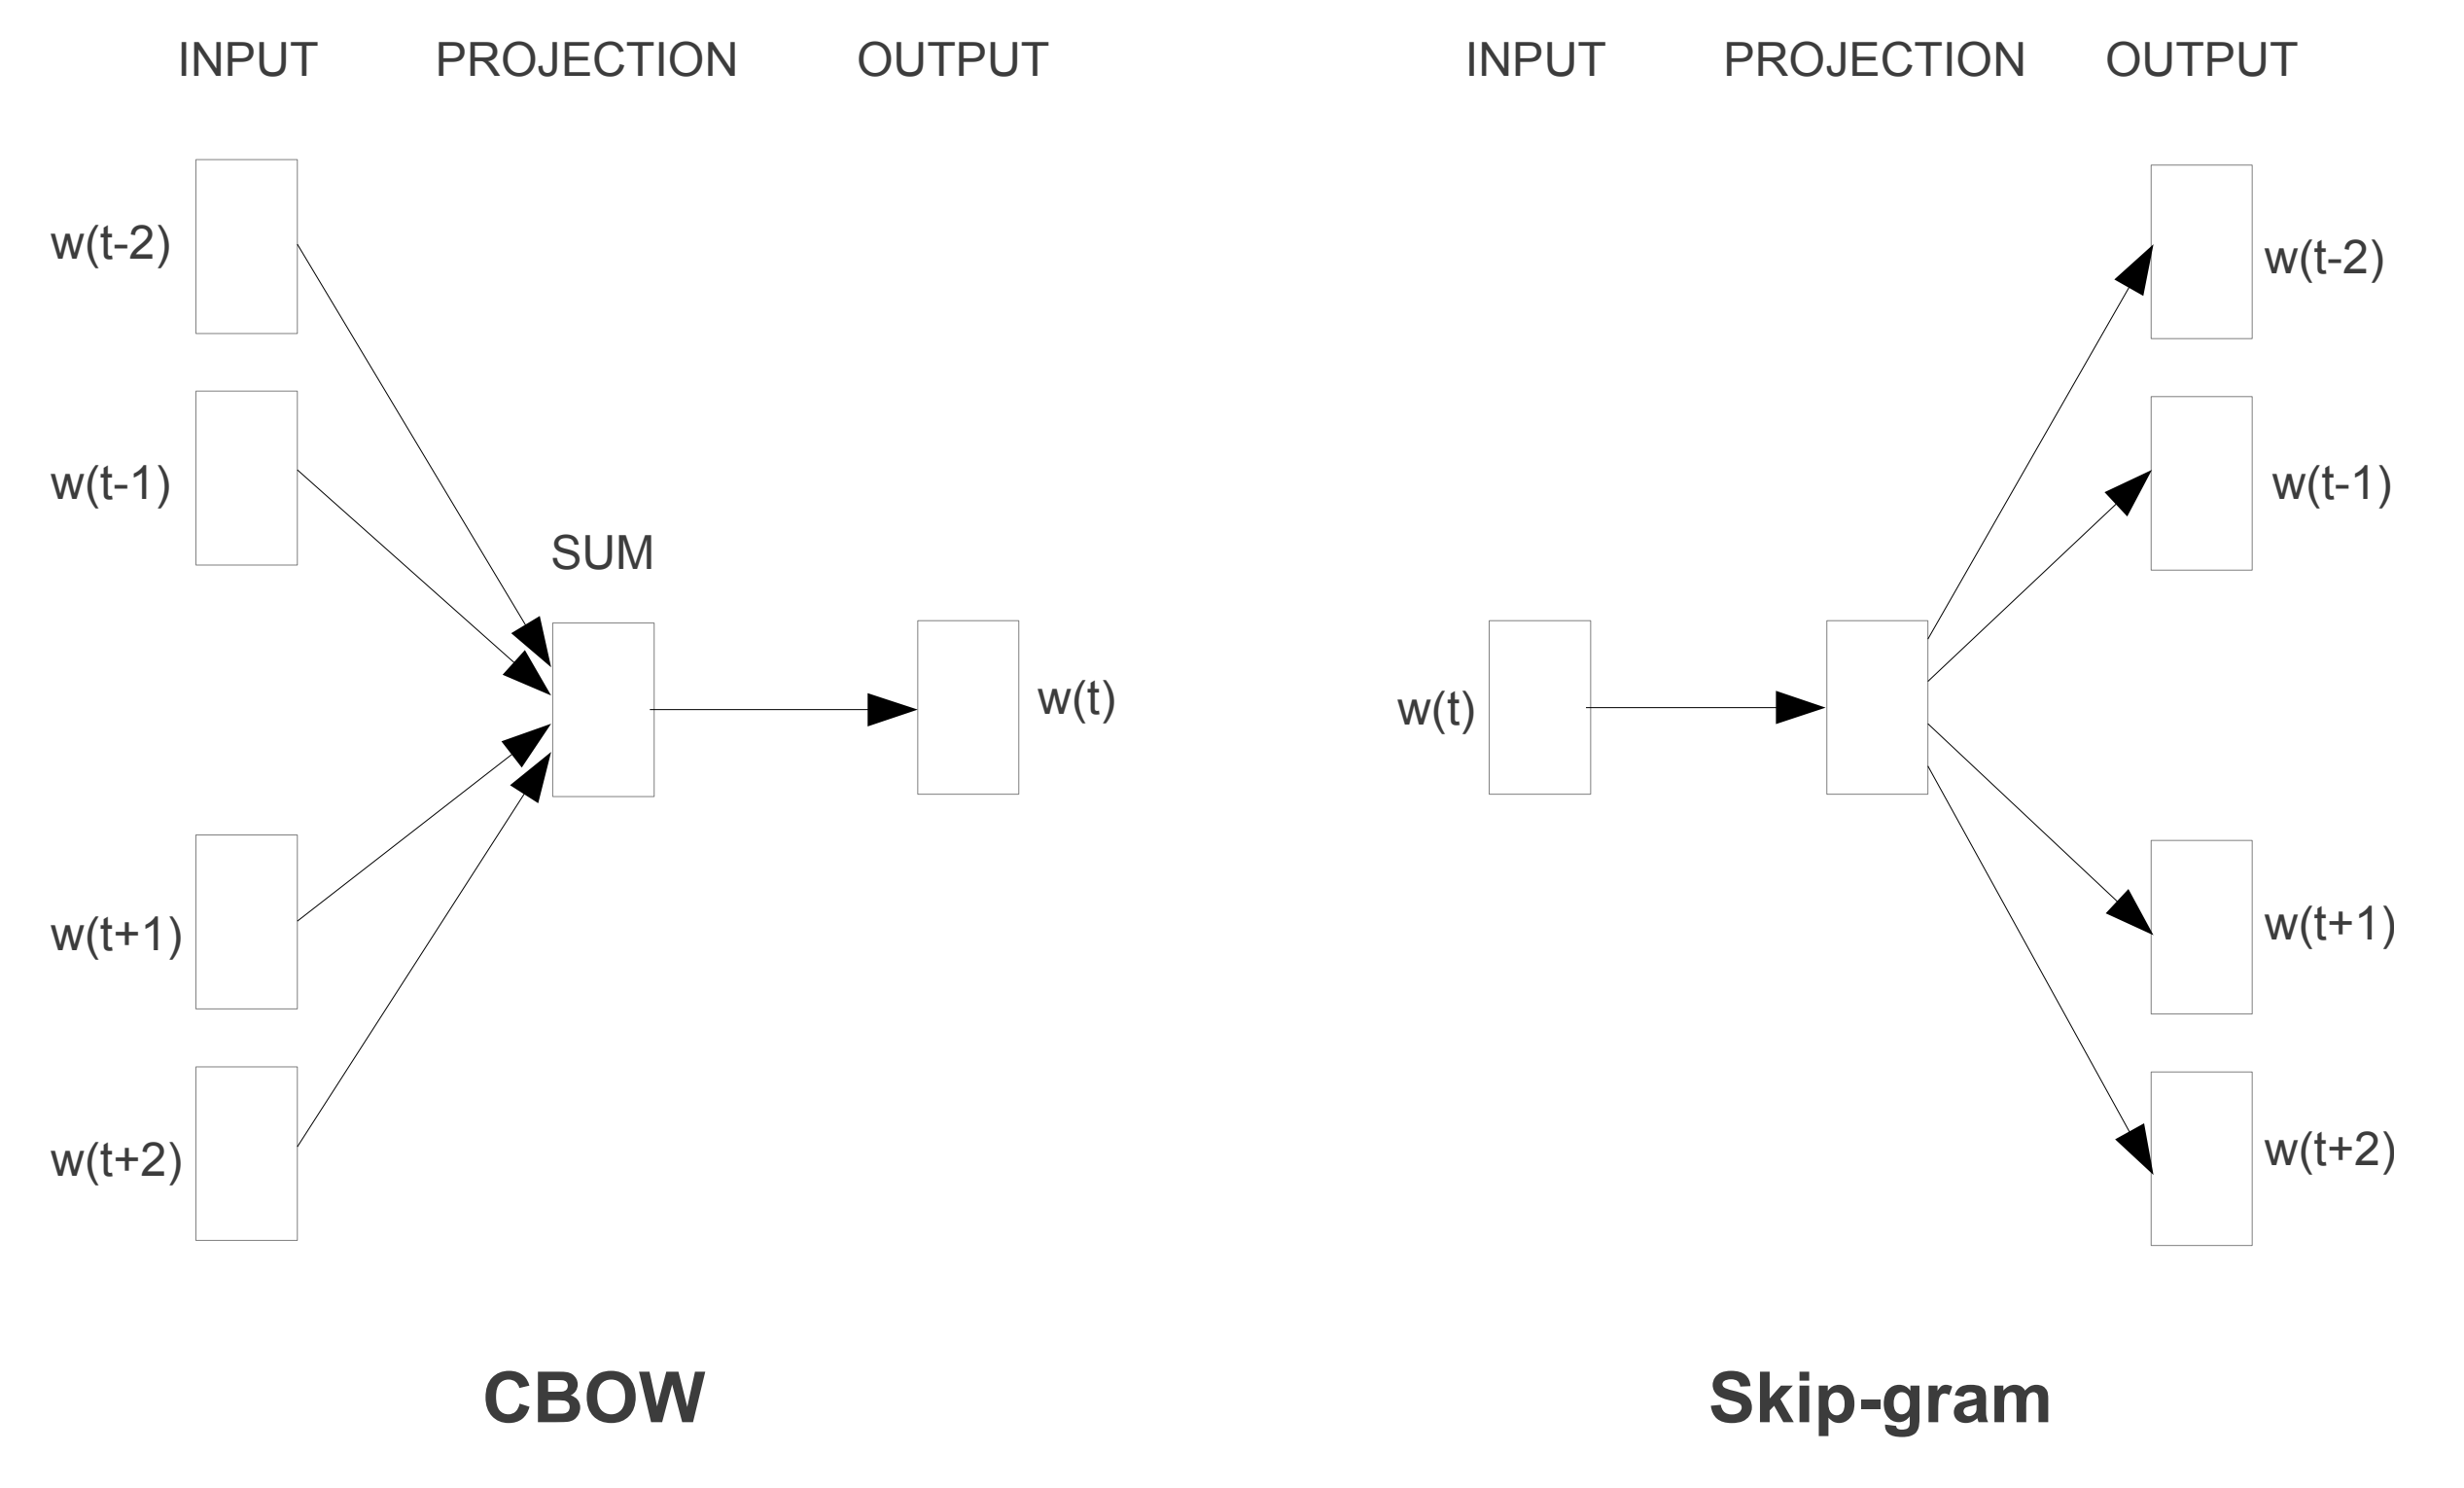
\includegraphics[width=0.7\linewidth]{sources/related_works/imgs/word2vec.png}
  \caption{Schema of the two Word2Vec training strategies. (from \citet{word2vec})}
  \label{fig:word2vec}
\end{figure}

\subsection{GloVe} 
\textit{GloVe} (Global Vectors for Word Representation) was introduced in \citet{pennington-etal-2014-glove}. Inspired by the rationale of PMI, they propose to learn a log-bilinear regression on a regularized co-occurrence matrix. Namely, they learn token representations $x$ and $\tilde{x}$ by optimizing the following objective\footnote{In practice, a regularization term is used to account for rare co-occurences.}:
$$
\argmin_{x, \tilde{x}} \sum_{i, j} (\langle x_i, \tilde{x}_j \rangle + b_i + b_j - \ln P_{ij})^2
$$
The authors conduct a variety of evaluation tasks and conclude that GloVe representations are more expressive than the ones obtained using CBOW or Skip-gram models.

\subsection{FastText}

FastText \citep{bojanowski-etal-2017-enriching} is an extension of Word2Vec where the token embeddings are enriched by character-level information to enhance their generalization abilities. The method is motivated by the inability of previous methods to cope with out-of-vocabulary strings, and an intent to facilitate the learning of semantic relationship for morphologically rich languages such as English where prefixes, suffixes and inflected forms are common. To that end, they represent tokens as a sum of substring representations of varying length, including the token string itself, and use the Skip-gram objective from Word2Vec at token-level over the summed representations. 

As a result, their token embeddings are more performant when it comes to identifying syntactic similarities between tokens, and representations can still be provided for unseen tokens.

Apart from building meaningful token representation spaces, these methods have been implemented into task-specific RNNs as a way to initialize or define look-up tables for input embeddings \citep{lstm_w2v, MUHAMMAD2021728}, yielding better results especially in low-resource scenarios.

\subsection{Contextual Embeddings}

Thanks to substantial progress in computational capabilities \citep{owens_gpu}, it became increasingly feasible to train large neural models using self-supervised methods on large amounts of text. Following the principles of transfer learning \citep{tl_survey}, intermediate representations of trained neural language models based on RNNs or Transformers were used as \textit{contextual} embeddings for task-specific model. 

\citet{peters-etal-2018-deep} extract the output vectors of the last LSTM layer of their frozen ELMo language model and use them as inputs for various task-specific sequential architectures. This leads to substantial improvements across most evaluations. Building upon Transformer-based language models, \citet{devlin-etal-2019-bert} and \citet{Radford2018ImprovingLU} simplify this framework and propose to replace the language modeling head by a task-specific untrained linear layer. The resulting architecture is then trained as a whole on the downstream task. This second training step is usually called fine-tuning, as it is often performed with finer optimization hyper-parameters.

\citet{martin-etal-2020-camembert} train a Transformer-based masked language model (MLM) on French data and compare its performance on downstream task with two settings: one where the pretrained model is frozen and a simple model is trained on top of it, and one where the model is fine-tuned on the downstream task. Although the frozen setting leads to slightly better performance in NER when combined with a LSTM-CRF \citep{panchendrarajan-amaresan-2018-bidirectional}, the fine-tuned model outperforms its frozen counterpart in most tasks, notably in Part-of-Speech tagging.

On word similarity tasks, these contextual representations were shown to better embed semantic similarity \citep{bommasani-etal-2020-interpreting}.



\section{Sentence Embeddings}
\label{sec:rw_sent_embs}
The contextual representations extracted from pretrained language models are also useful to evaluate sentence similarity in a zero-shot setting when building metrics from token-level similarity \citep{Zhang2020BERTScore}. 

However, \citet{reimers-gurevych-2019-sentence} show that building sentence-level representations using basic pooling strategies (e.g. using the representation of one token only or averaging the representations over the sequence) performs better when using static embeddings such as GloVe than with these contextual representations. Their work paves the way for specialized methods that build expressive sentence embeddings from neural contextual representations.

\subsection{Sentence-BERT}
\begin{figure}[ht]
  \centering
  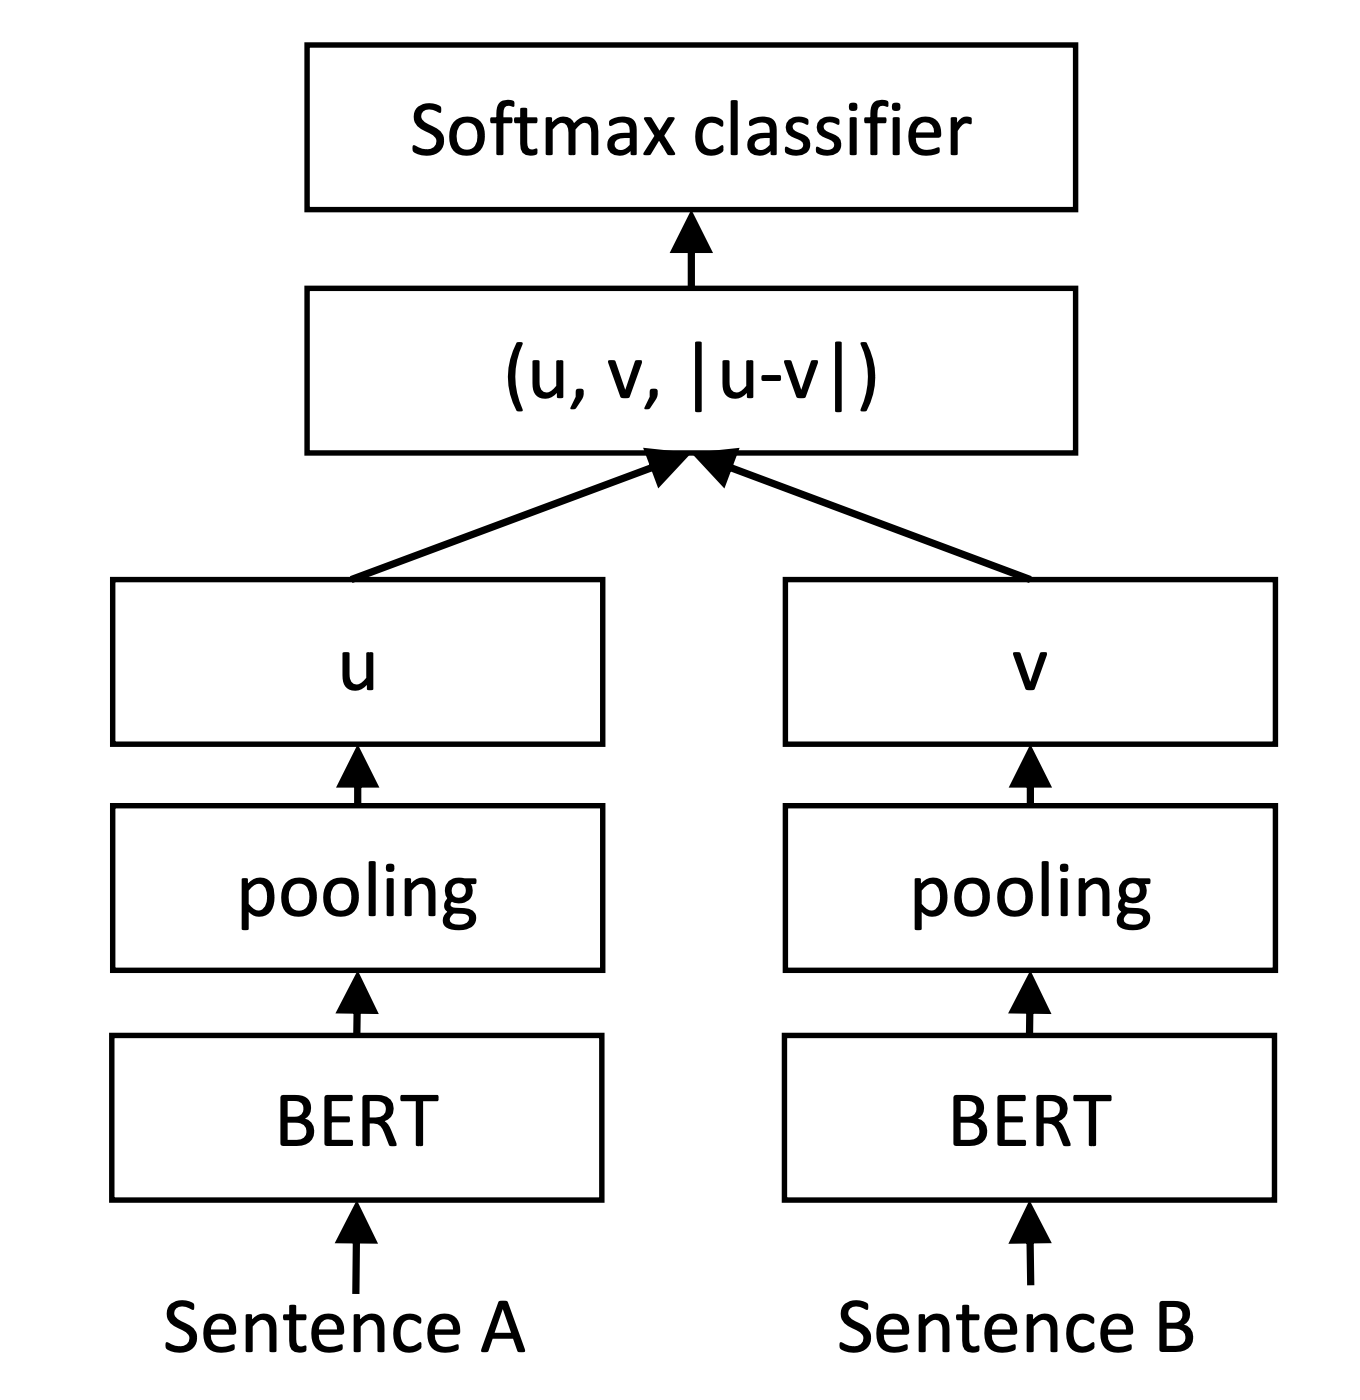
\includegraphics[width=0.3\linewidth]{sources/related_works/imgs/sbert.png}
  \caption{Overview of the Sentence-BERT training paradigm (taken from \citet{reimers-gurevych-2019-sentence})}
  \label{fig:sbert}
\end{figure}

\citet{reimers-gurevych-2019-sentence} introduce Sentence-BERT, a model based on BERT that generates sentence-level representations. They use a siamese architecture where a single model encodes two sentences into pooled representations, and a classifier predicts a label that should detect whether two sentences share the same meaning. This siamese network is initialized with BERT or RoBERTa models and is further trained on the SNLI dataset \citep{hill-etal-2016-learning}, a \textit{natural language inference} (or NLI) dataset that comprises pairs of sentences associated with a label indicating a semantic correspondance between the sentences. At inference time, the siamese network produces sentence embeddings and their \textit{cosine similarity} is computed as a similarity score.

Cosine similarity is a vector space metric based on cosine distance that measures the angular discrepancy between two vectors. Given two vectors $x, y \in \mathbb{R}^d$, their cosine similarity is defined by:
$$
\text{cos-sim}(x, y) = \frac{\langle x, y \rangle}{||x||_2 \cdot ||y||_2}
$$
Thus, $\text{cos-sim}(x, y) \in [-1, 1]$ and higher cosine similarity values depict vectors which directions are more aligned.

They evaluate their model against concurrent work such as USE \citep{cer-etal-2018-universal} and InferSent \citep{conneau-etal-2017-supervised} on the Sentence Textual Similarity (STS) benchmarks that provide sentence pairs with semantic similarity scores. Using the Spearman correlation metric \citep{zar2005spearman}, they show that the cosine-similarity between the Sentence-BERT representations correlates significantly better with the ground-truth similarity scores compared with other approaches.

Similar supervised methods have been applied with multilingual and/or multimodal data and base models to obtain language-agnostic sentence representations \citep{feng-etal-2022-language}. Concurrently, \citep{schwenk-douze-2017-learning} propose to learn multilingual sentence representations by training monolingual sentence encoders and decoders for machine translation. This approach was later successfully adapted to multi-modal representations \citep{Duquenne:2023:sonar_arxiv}.


\subsection{Latent Regularization Methods}

The contextual representations of pretrained LMs are trained in a way that implicitly forces them to capture syntactic and semantic information at token-level \citep{jawahar-etal-2019-bert}. Nevertheless, their geometrical structure is not constrained by any explicit process, and it remains unclear whether their final structure can be predicted \textit{a priori}.

As we will discuss in the next section, this structure can be strongly degenerate in practice, which makes pooling nicely distributed sentence representations a more difficult task. Aware of this difficulty, several methods have been proposed to regularize the token-level representation distributions before pooling, in order to lead to sentence embeddings for which cosine similarity is more expressive.

\citet{arora2017a} and \citet{mu2018allbutthetop} remove the most dominant principal components of the SVD of token-level representations, and observe improvements in the expressiveness of the resulting sentence embeddings. \citet{li-etal-2020-sentence} take a different stance and train a flow-based generative model that maps the contextual token embeddings to a standard Gaussian distribution. Their BERT-flow model improves over the average-pooling baseline in most STS benchmarks. \citet{su2021whiteningsentencerepresentationsbetter} propose a more direct approach and learn a \textit{whitening} transformation, an affine mapping that gives the contextual distribution the same first two moments as the standard multi-dimensional Gaussian distribution (i.e. $\mu = 0_d$ and $\Sigma = I_d$).

\subsection{Contrastive Methods}
\label{ssec:contrastive}

Although siamese networks and latent regularization are both ways to improve representations taken from pretrained LMs, these methods are incompatible. As a matter of fact, the former retrains the model without constraining the geometry of the token (and sentence) embeddings, while the latter performs expensive \textit{post-hoc} regularizations that may be non-differentiable and that are not designed to be applied at every training step.

As a result, it is difficult to both benefit from the geometrical regularity of the intermediate representations (or their \textit{uniformity}) which allows the model to differentiate properly different samples, and from the capacity of these representations to accurately capture the information in the sentences and match similar sentences (or their \textit{alignment}).

\citet{pmlr-v119-wang20k} design metrics to quantify alignment and uniformity in representations, and empirically show that the most expressive representation tend to optimize both metrics. They proceed to prove that \textit{contrastive learning} objectives implicitly lead to a trade-off between alignment and uniformity.

Contrastive Learning is a representation learning framework that aims at learning discriminative embeddings by using objectives that minimize the underlying distance between equivalent items (\textit{positive} pairs) and maximize it between unrelated items (\textit{negative} pairs). A crucial design choice in contrastive learning methods is the definition of equivalence between the considered items, especially in the unsupervised setup. In computer vision, building positive samples is relatively easy as slight perturbations of the input features do not affect the human perception of the resulting image. This made contrastive learning particularly convenient, leading to several popular models \citep{simclr, He_2020_CVPR}.

\begin{figure}[ht]
  \centering
  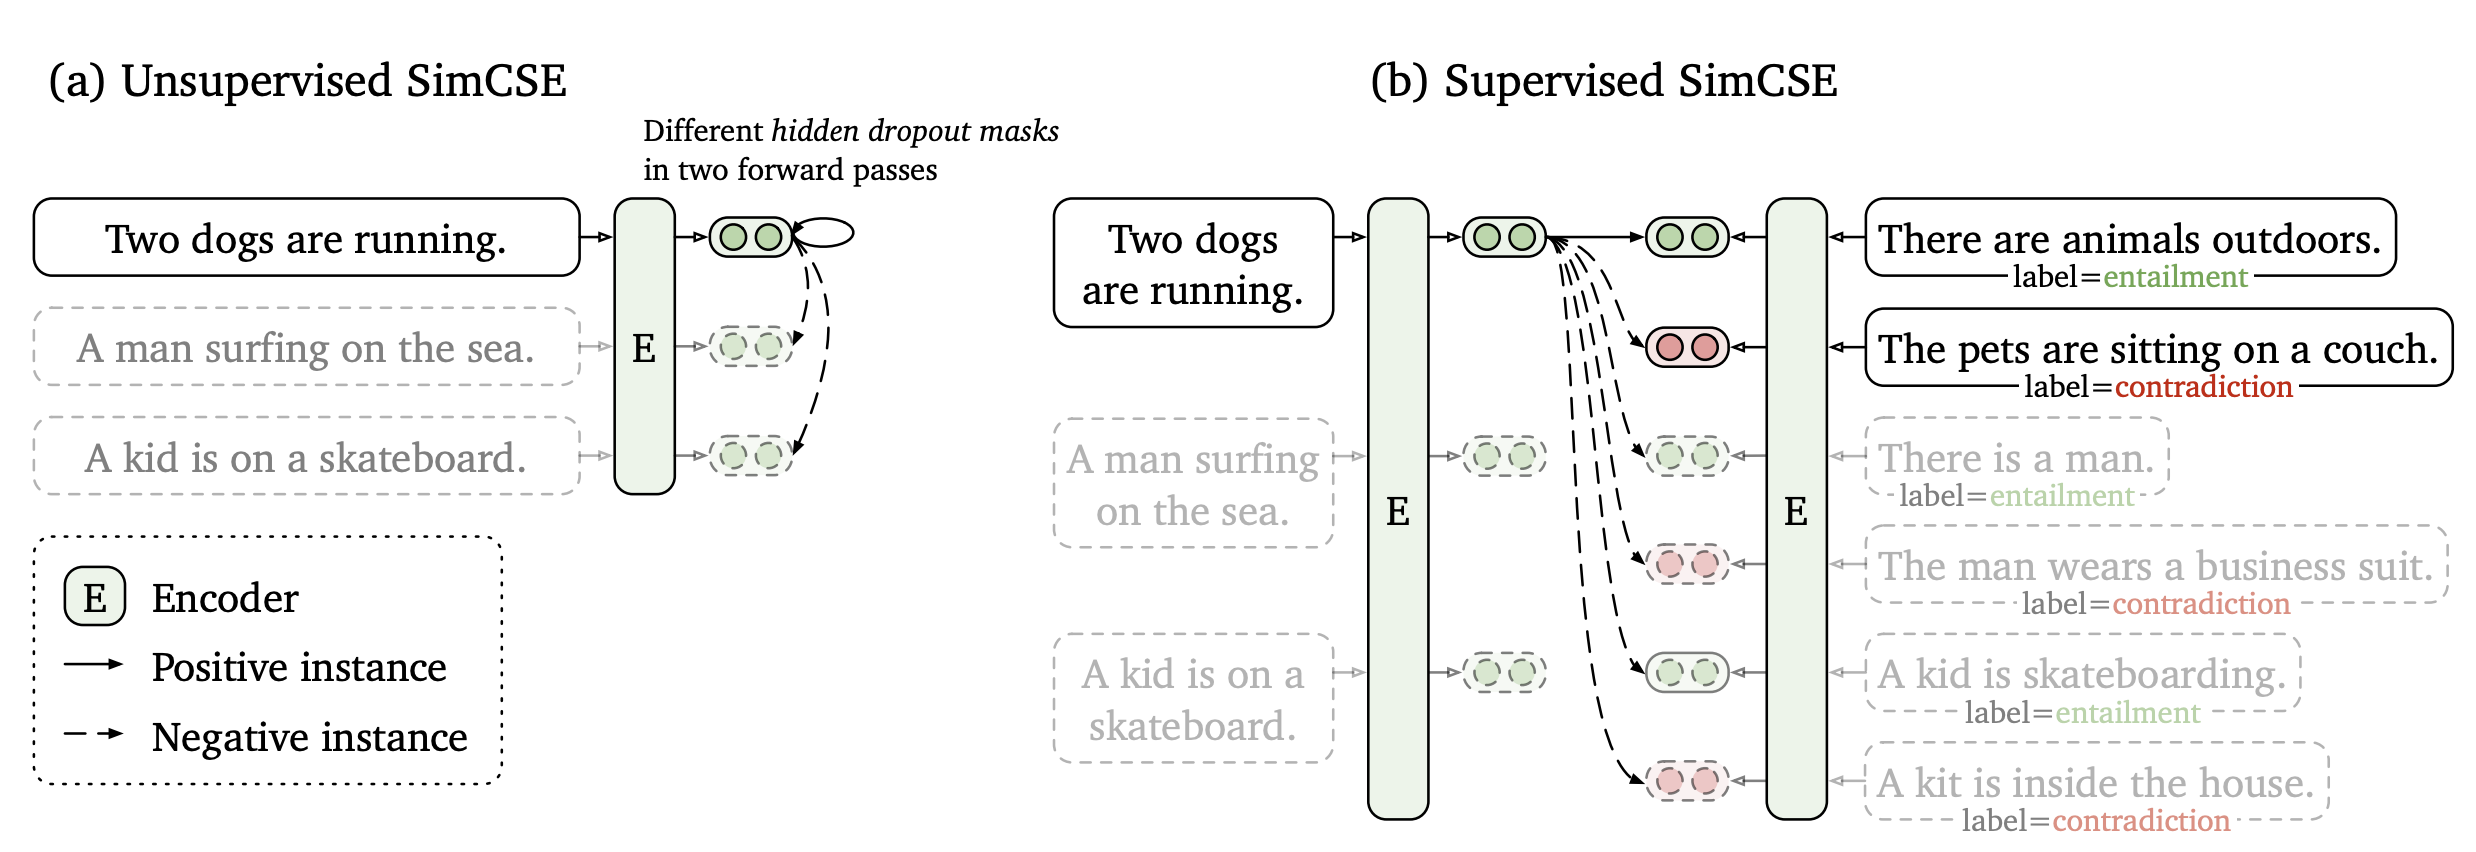
\includegraphics[width=0.9\linewidth]{sources/related_works/imgs/simcse.png}
  \caption{Overview of the SimCSE contrastive unsupervised and supervised frameworks (from \citet{gao-etal-2021-simcse})}
  \label{fig:simcse}
\end{figure}

Inspired by contrastive methods, and to improve the uniformity-alignment tradeoff, \citet{gao-etal-2021-simcse} develop the SimCSE models. They first apply a classical contrastive learning objective to sentence-level representations in a supervised setting. Many NLI datasets provide several sentence pairs for a given sentence, each matching it with a similar sentence or one with an opposite meaning. Hence, \citet{gao-etal-2021-simcse} leverage these pairs tagged as similar as positive samples, and those tagged as dissimilar as negative samples. They also use sentences from unrelated pairs as additional negative samples. 

Similarly to \citet{simclr}, they leverage the InfoNCE objective \citep{oord2019representationlearningcontrastivepredictive} which can be interpreted as a cross-entropy loss on in-batch classification, i.e. identifying the object in a training batch to which a representation corresponds. Formally, given an object embedding $h \in \mathbb{R}^d$, a positive sample embedding $h_+ \in \mathbb{R}^d$ and a series of negative samples $h^i_- \in \mathbb{R}^d$ for $i \in [1, N_-]$, the InfoNCE objective based on cosine similarity is:
$$
\mathcal{L}_{\text{InfoNCE}} = \mathbf{E}_{h, h_+, \mathbf{h}_-}\left(-\log \frac{\exp \text{cos-sim}(h, h_+)}{\exp \text{cos-sim}(h, h_+) + \sum_{i=1}^{N_-} \exp \text{cos-sim}(h, h^i_-)}\right)
$$

In the supervised SimCSE, $\mathbf{h}_-$ contains representations corresponding to the dissimilar utterance as annotated in the NLI dataset, and the other sentences from the same training batch. This dissimilar utterance constitutes a \textit{hard} negative as it should be particularly be contrasted with the target sentence, as opposed to the soft negatives that should statistically be neutral with respect to the target sentence. \citet{gao-etal-2021-simcse} also provide an unsupervised approach where $\mathbf{h}_-$ does not contain the hard negative from the NLI annotation. In this setting, as the positive NLI sample is not available, they need to resort to data augmentation in order to provide a similar utterance. In NLP, such augmentation can be hard to design safely, as altering one token can change the meaning of the whole sentence. Nevertheless, some attempts have been made to edit the token sequence (\citet{10.1145/3593590} for instance). \citet{gao-etal-2021-simcse} avoid this difficulty by computing the sentence representations twice using a different dropout filter.

\citet{gao-etal-2021-simcse} conduct experiments and drastically outperform models in both the latent regularization and the siamese network frameworks, and they show that SimCSE achieves a much more balanced alignment-uniformity tradeoff. SimCSE paved the way for contrastive methods in sentence-level representation learning, with subsequent works that improved the negative sampling strategies \citep{yan-etal-2021-consert}, scaled the training process and data \citep{li2023generaltextembeddingsmultistage}, making it the state-of-the-art approach for sentence embeddings.

\vspace{2em}

Overall, we have seen in this section how learning representations of textual data can bring a specific set of challenges, as naively applying general methods often fails the test of linguistic complexity. As the potential offered by machine learning methods increased, these methods have often shown to benefit from tweaks specific to the text modality that helped improve the downstream performance of NLP systems.

As downstream and language modeling performances become more and more intertwined, this naturally raises the question of whether neural language models are also affected internally by the same kind of phenomena, and leads us to analyzing their representations in order to characterize the impact of textual data on their geometry.

\newpage